\documentclass[11pt,a4paper]{article}
\usepackage[spanish]{babel}
\usepackage{graphicx}
\graphicspath{{imagenes1/}}
\usepackage{amsmath}
\usepackage{amssymb}
\usepackage{mathrsfs}
\usepackage{cancel}

\begin{document}
\begin{center}
\textbf{REPORTE DE PRACTICA}\\
CIRCUITOS DE RECTIFICACION NO CONTROLADOS
\end{center}

\begin{center}
Ascencio De Leon Agustin\\
12-sep-2019\\
Universidad Politecnica de La Zona Metropolitana de Guadalajara
\end{center}

\section{Objetivo de la practica}
Saber el funcionamiento de cada rectificador y cuales caracteristicas las diferencian entre cada una de ellas.

\section{Procedimiento}
\subsection{Rectificador de media onda con carga inductiva.}
Esta nos permite poner de manifiesto algunos de los conceptos elementales de rectificacion no controlada:

\begin{figure}[h]
\centering
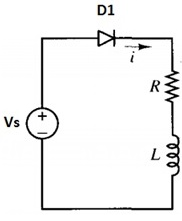
\includegraphics[scale=.4]{1.png} 
\end{figure}

Ya teniendo la simulacion en orcad, en la siguiente figura se mjestra como la onda de la tension rectificada se aplica a la carga.\\
Como se observa, la tension de salida no se anula hasta que no lo hace la corriente de carga, lo que significa que el diodo rectificador permanece polarizado en directo incluso durante una porcion del semiperiodo negativo de la tension de entrada.\\
\newpage Esto es debido a que la indutancia de salida se opone a variaciones bruscas de corriente y asi crea una sobretension necesaria para mantener al diodo en conduccion hasta que la corriente sea nula.

\begin{figure}[h]
\centering
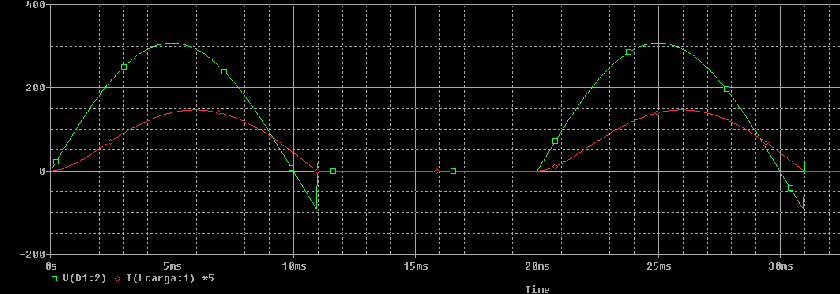
\includegraphics[scale=.4]{2.png} 
\end{figure}

\subsection{Tension y corriente en el diodo rectificador.}

\begin{figure}[h]
\centering
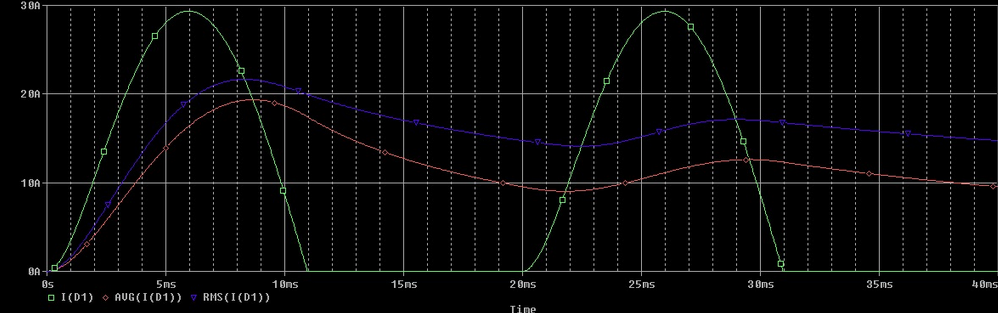
\includegraphics[scale=.4]{3.png} 
\caption{Tension y corriente en el diodo rectificador}
\end{figure}

\subsection{Tension en el diodo rectificador.}

\begin{figure}[h]
\centering
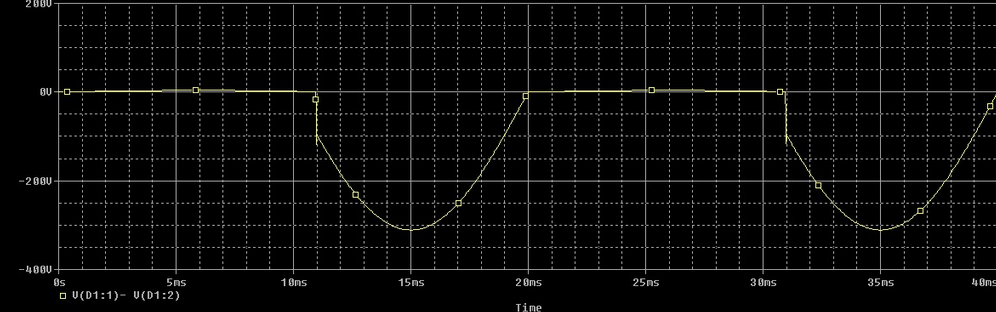
\includegraphics[scale=.4]{4.png}  
\end{figure}

Es necesario poner en PSPICE las caracteristicas que tiene cada una de las ondas que vienen en el manual de practica.

\subsection{Rectificador monofasico en puente.}

\begin{figure}[h]
\centering
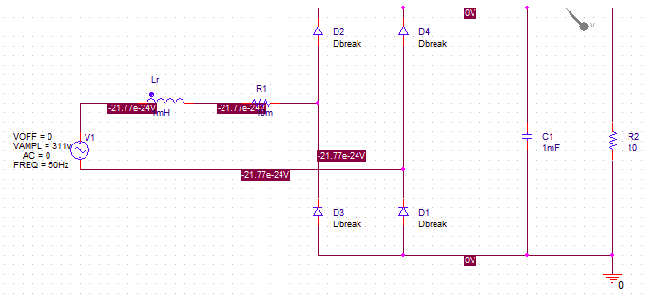
\includegraphics[scale=.4]{5.png}  
\caption{Rectificador de media onda con carga RL}
\end{figure}


El rectificador monofasico o puente de diodos, la etapa de continua consta de un filtro constituido por los elementos Cf y Lf , destinado a atenuar el rizado de la tension de salida. En la etapa de alterna se han añadido los elementos Rr y Lr para tener en cuenta la resistencia y la inductividad de la red vistas desde el rectificador.\\
En este circuito podremos estudiar las principales formas de ondas que caracterian su funcionamiento y determinan la eleccion de los diodos empeorando el factor de potencia.

\begin{figure}[h]
\centering
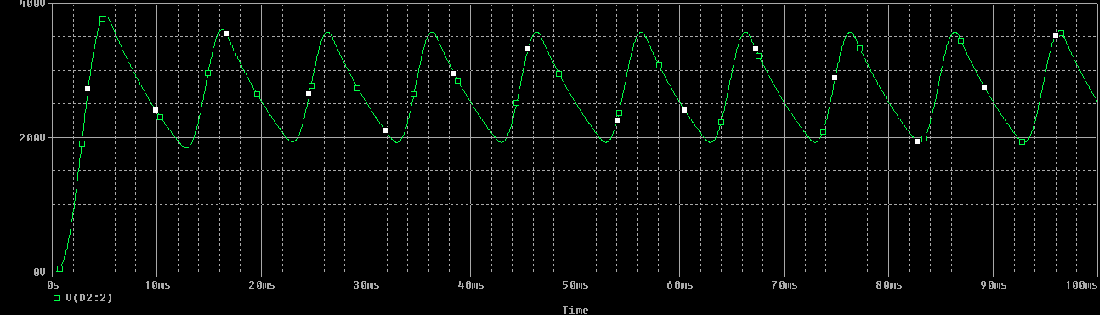
\includegraphics[scale=.15]{6.png} 
\end{figure}

\subsection{Tension y corriente de entrada del rectificador.}

\begin{figure}[h]
\centering
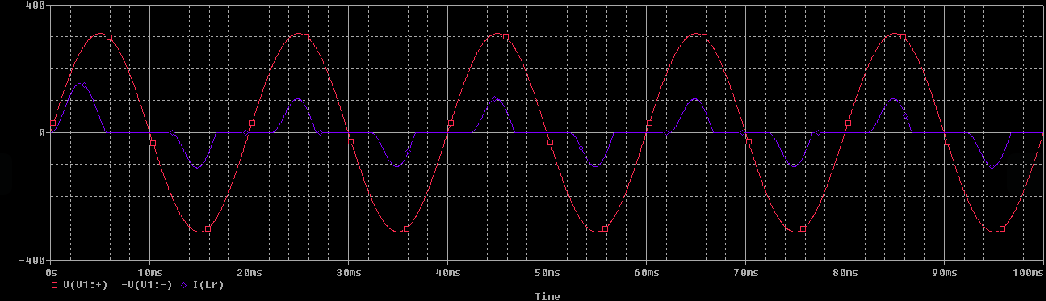
\includegraphics[scale=.5]{7.png} 
\end{figure}

\subsubsection{Distorcion de la corriente de entrada.}
Ya teniendo en claro como trabajaba la tension y la corriente de un rectificador haremos el uso de cuantificacion de las observaciones precedentes y determinar el factor de potencia globaldel rectificador, utilizando los \textbf{RESULTADOS DEL ANALISIS DE FOURIER} una herramienta que nos da PSpice en tabla en el fichero de salida (\emph{out.}) en el programa.\\

\begin{figure}[h]
\centering
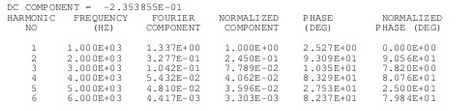
\includegraphics[scale=.3]{8.png} 
\end{figure}

Gracias a esta tabla se recogen los coheficientes de \emph{Fourier} que responden a la siguiente expresion:

$$ i_{Lr} (t) = C_{o} + \sum_{n=1}^{\infty} C_{n} sen(nw * t+ \cancel{o}_{n} ) $$

Cuando:\begin{enumerate}
\item $ C_{o} $ = La componente de continua de la forma de onda analizada.
\item $ C_{n} $ = La amplitud del armonico de orden
\item $ \cancel{o}_{n} $ = La fase correspondiente respecto a la referencia (determinado por la tension de red)
\end{enumerate}

Por lo tanto en este analisis la distorcion armonica total de la corriente es de 80 porciento, en tanto que el angulo de desfase entre la tension, la red y la componente fundamental de la corriente es $ \cancel{o}_{1} = 3,97 $, lo que nos da como resultado un factor de potencia de desplazamiento de valor:

$$ DPF = cos\cancel{o}_{1} = cos3,97 = 0,998 $$

Y asi la Formula para sacar el factor de potencia global es:

$$ PF = \dfrac{DPF}{\sqrt{1 + TDHi^2}} = \dfrac{0,998}{\sqrt{1 + 0,8^2}} = 0,779 $$

Como en esta practica la potencia es baja significa que se absorbe una cantidad de potencia reactiva de la red 

Los resultados del analisis de Fourier permiten dibujar en \emph{Probe} la componnte fundamental de la corriente de entrada y la corriente de distorcion, definida como la diferencia entre la forma real y la correspondiente a la componente fundamental.\\
\\
Para eso, utilizando los operadores de \emph{Probe} introduciremos la siguiente ecuacion:

$$ i_{1} = 51.67 * sin(314*time + 0.069) $$

donde por coherencia con el resto de unidades, el valor de $ \cancel{o}_{1} $ debe introducirse en radianes y no en grados.

\begin{figure}[h]
\centering
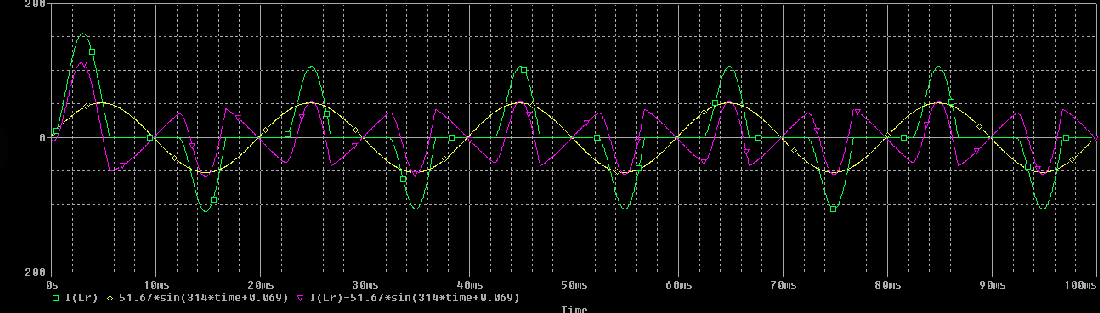
\includegraphics[scale=.4]{9.png} 
\end{figure}

\subsection{Rectificador monofasico duplicador de tension.}
Tal y como lo muestra en el manual haremos uso de orcad nuevamente para simular el siguiente circuito:

\begin{figure}[h]
\centering
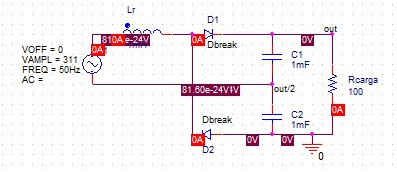
\includegraphics[scale=.5]{10.png} 
\end{figure}

Este tipo de rectificador permite obtener en la salida una tension que corresponde aproximadamente al doble de la que se obtiene en el circuito de \textbf{Distorcion de la corriente de entrada}. Obteniendo asi tensiones elevadas en la etapa continua sin necesidad de utilizar tranformador que eleve la tension de entrada del rectificador.

\subsection{Rectificadores monofasicos en lineas trifasicas.}
Ilustrando un conjunto de 3 receptores monofasicos de igual potencia conectados entre cada una de las fases y el neutro de la instalacion. El simbolo del manual corresponde a un \textbf{subcircuito} que viene a continuacion:

\begin{figure}[h]
\centering
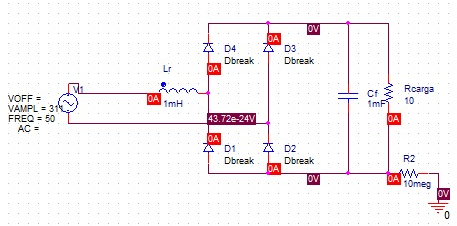
\includegraphics[scale=.5]{11.png} 
\end{figure}
 
\textbf{Nota:} En este circuito conectamos una fuente como indicador de la coneccion al circuito original.

\begin{figure}[h]
\centering
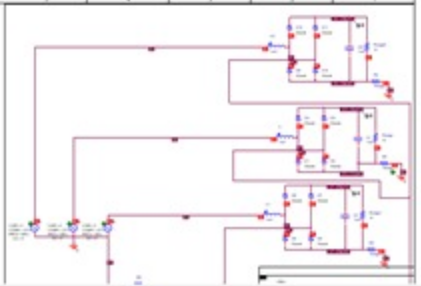
\includegraphics[scale=.5]{12.png} 
\end{figure}

\subsection{Rectificador Trifasico.}
Al igual que los demas receptores electricos, los rectificadores trifasicos  son utilizados cuando la potencia de la red es consumida de manera elevada, ya que en estos casos la utilizacion de rectificadores monofasicos provocarian desequilibrios importantes en el consumo de las fases.\\
Por lo tanto de nuevo haremos el uso de las simulaciones en \textbf{Orcad} para mostrar de manera mas efectiva el funcionamiento de un rectificador monofasico no controlado:

\begin{figure}[h]
\centering
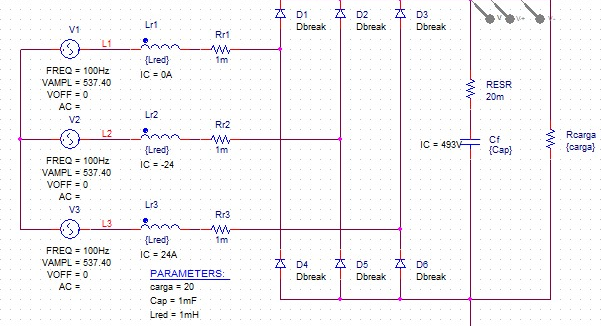
\includegraphics[scale=.6]{13.png} 
\end{figure}

Los cuales sus parametros a cargar seran los siguientes:
\begin{enumerate}
\item Carga 20ohms
\item Cap 1mF
\item Lred 1mF
\end{enumerate}

Estos parametros seran utilizados y hechos buscando en la biblioteca el componente \textbf{PARAM} y de ahi haciendo doble click te saldra un pequeño cuadro donde pondras esas tres caracteristicas.\\
Para esto a los componentes (\textbf{Resistencia,Capacitor y Bobina}) les pondras en donde van sus respectivos valores los parametros de la lista anterior.

\subsection{Efecto de las inductancias de red sobre la conmutacion de corriente.}

\begin{figure}[h]
\centering
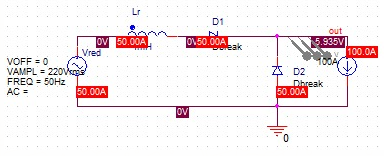
\includegraphics[scale=.5]{14.png} 
\end{figure}

En este circuito en ausencia de inductancia de red, cuando la tension de entrada fuese positiva al dioso 1 se polariza en directoy conduciria. De lo contrario el diodo 2 estaria polarizado a la inversa y estaria bloqueando.\\
En lo que la tension de salida se refiere, la forma de onda resultante seria casi nula durante la conduccion del diodo 2.\\
Durante todo ese tiempo de salida permanece cortocircuitada por el diodo 2, produciendose la perdida de tension como se mira en la onda de \textbf{PSPICE} en \textbf{ORCAD}:

\begin{figure}[h]
\centering
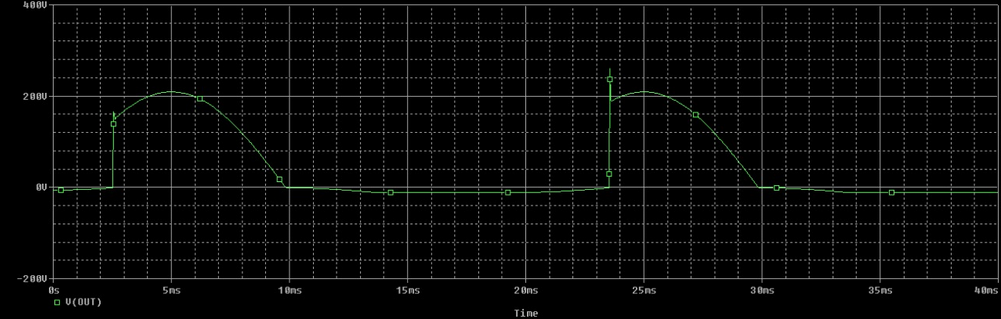
\includegraphics[scale=.3]{15.png} 
\end{figure}

Se demuestra que la perdida de tension media en la carga se calcula de la siguiente manera:

$$ \nabla V_{o} = \dfrac{w*L_{r}}{2\pi} * I_{o} $$

\begin{figure}[h]
\centering
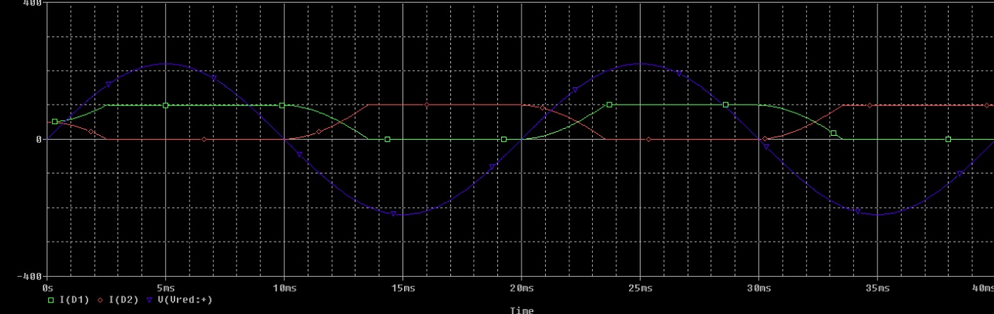
\includegraphics[scale=.3]{16.png} 
\end{figure}

\begin{center}
\section{Conclusion}
En esta practica se tuvo en cuenta datos ya vistos en anteriores cursos, reforsando asi la utilidad de ciertos circuitos en instalaciones electricas y su practicidad en el alacenaje y concentracion de energia electrica, dando como resultado circuitos simples pero muy utiles encuanto a la practica, dando base a mas conocimientos futuros, en los circuitos de la practica se demuestra la eficiencia de los mismos en las señales senoidales y de media onda. 
\end{center}

\end{document}